\section{What you will build}
Wave 1 starts with two parked UAVs. They ascend to model-origin height 2.8 m, cross toward opposite destination pads and descend. Both take off simultaneously. When a one-second prediction detects an approaching conflict, UAV 2 holds in flight and gives UAV 1 priority. It resumes at the first update where the remaining crossing legs have sufficient predicted clearance. Wave 2 adds a stationary red sphere. Each UAV follows a bypass on its own side and then crosses to the opposite destination pad using the same priority rule.

The four mission stages are READY, TAKEOFF, TRAVEL/BYPASS and LANDING. YIELD is a deliberate wait in both waves. LANDED denotes arrival; COMPLETE requires both vehicles to have arrived. FAILED denotes a detected problem. A timeout is not successful obstacle avoidance.

\begin{figure}[htbp]\centering
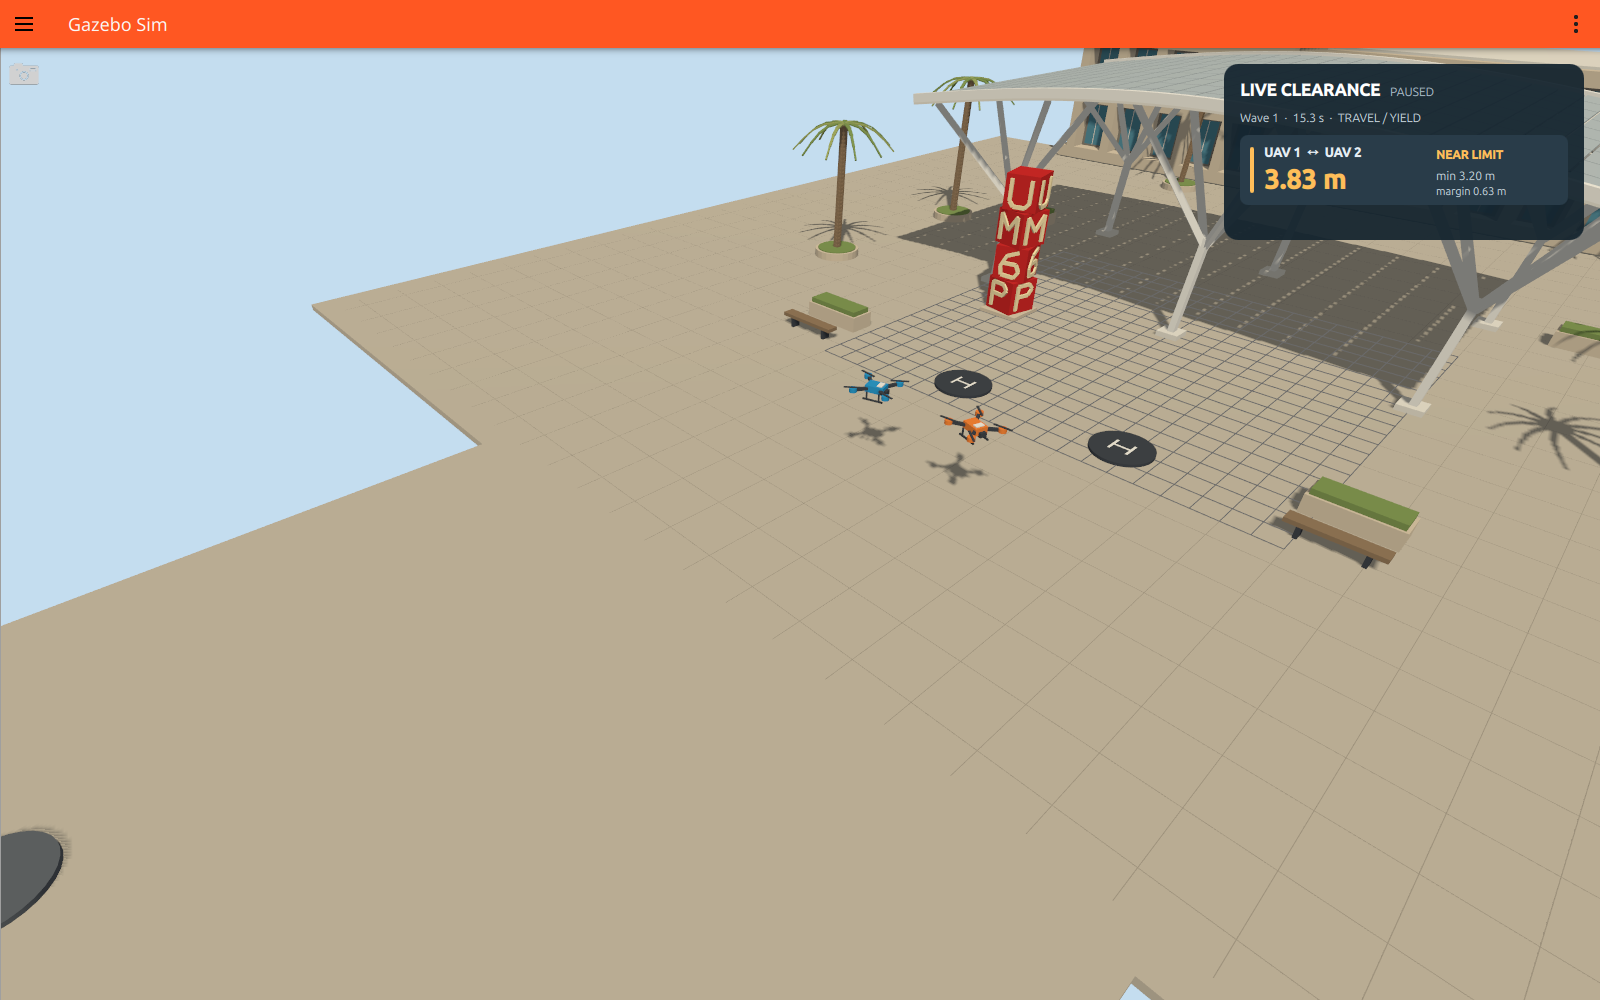
\includegraphics[width=.94\linewidth]{assets/wave1.png}
\caption{Actual Gazebo Wave-1 rendering during the pause/resume verification. The orange vehicle yields while the blue vehicle proceeds. The live counter shows measured separation.}
\end{figure}

The original paused environment remains available through its original launcher. Each demonstration has its own package and uses a separate world named \texttt{um6p\_demo}. Its motion plugin is absent from the paused world. Only the new demonstration advances simulation time after an explicit start command.

\section{Software and prerequisites}
ROS 2 runs the launch process and receives telemetry. Gazebo owns the scene, simulation clock and model positions. \texttt{ros\_gz\_bridge} translates Gazebo state messages and clock messages into ROS messages. A workspace contains packages; building a package installs its files so launch can resolve them by package name. An SDF file describes the world. A C++ system plugin runs inside Gazebo's update loop.

The tested native stack is Ubuntu 24.04.5 amd64, ROS 2 Jazzy, Gazebo Harmonic Sim 8.15.0 and ros\_gz 1.0.24, with Intel Iris Xe/Mesa hardware rendering. The installation already existed; no driver or system upgrade was performed. This is the same supported pairing as the campus preparation. Earlier user-reported patch versions, a freshly provisioned OS, Docker and software-only rendering are not claimed tested.

Prerequisites: the complete updated delivery folder, a Bash terminal, the existing ROS/Gazebo installation, a C++ compiler and colcon. GUI commands additionally need a working graphical desktop. The original native dependency list and the added demo dependency list record package requirements; observed versions are evidence, not a permanent apt lock. All project assets are local after setup. No runtime model download is required.

\section{Enter, build and inspect the workspace}
Commands in this guide are literal Bash commands except example paths, which you must replace. Do not type a shell prompt character. Quote paths containing spaces. Unless stated otherwise, work from the delivery root.

Working directory: any terminal initially. Purpose: enter the extracted folder and check installed prerequisites. Expected result: the check prints OS/tool versions and the plan reports missing dependencies or confirms they exist. These checks do not install software.
\begin{lstlisting}
cd "/your/path/ros2_gazebo_um6p_campus"
bash scripts/check_environment.sh
bash scripts/setup.sh --plan
\end{lstlisting}
The additive setup script checks both dependency manifests. To install missing packages on a compatible machine, from this same directory run \texttt{bash scripts/setup\_demo.sh --install-missing} after reviewing its plan. This requires sudo and configured official apt repositories; expected result is the missing packages installed without upgrading existing ones. This installation command was not needed on the tested machine. The new C++ package uses the existing \texttt{gz\_sim\_vendor} and \texttt{gz\_plugin\_vendor} development exports, plus Gazebo GUI and Qt 5 Quick development packages for the counter overlay. See \texttt{references/demo-packages.txt}. If they are absent, use the original tutorial's explicit installation procedure after reviewing the proposed apt transaction. Do not replace working ROS installations to follow this guide.

Working directory: delivery root. Prerequisite: dependencies present. Purpose: compile and install all five packages locally. Expected result: colcon reports five packages finished, including \texttt{um6p\_demo\_core} and both scenario packages.
\begin{lstlisting}
bash scripts/build.sh
\end{lstlisting}
Build and install products remain inside this workspace. Runtime uses copied installed assets and the installed shared library. Source changes require a rebuild. No personal shell configuration is required: the launch wrappers source ROS and this workspace explicitly.

\section{Run and record each wave}
Working directory: delivery root in Terminal A. Prerequisites: build succeeded and no other campus demonstration is running. Purpose: open Wave 1. Expected result: Gazebo opens with both UAVs parked and simulation time paused at zero. This command stays attached to Terminal A.
\begin{lstlisting}
bash scripts/launch_demo.sh 1 gui
\end{lstlisting}
Working directory: the same delivery root in Terminal B. Prerequisite: the scene has loaded. Purpose: start the demonstration clock and deterministic motion. Expected result: the service replies \texttt{data: true}; after three seconds of simulation time, ascent begins.
\begin{lstlisting}
bash scripts/demo_control.sh start
\end{lstlisting}
The start command is intentional. This phase was separately authorized to advance kinematic simulation time. The motion plugin reads simulation time, never wall-clock time, for motion. Pausing freezes both positions and mission progress. The following commands, each from Terminal B while Terminal A owns the scene, pause and resume it. Expected result: \texttt{data: true} each time.
\begin{lstlisting}
bash scripts/demo_control.sh pause
bash scripts/demo_control.sh resume
\end{lstlisting}
For a recording, first load the paused scene, position the camera using mouse navigation, start your desktop screen recorder, then issue the start command. Record until both UAVs land. You may pause to explain a view. The researcher supplied two original MP4 recordings, now preserved unchanged in the respective demo media/videos folders. The recording software and its exact capture settings were not independently verified. The screenshot figures in this guide came from Gazebo itself.

Shutdown: press \textbf{Ctrl+C once in Terminal A} and wait for clean child exit messages. To repeat from the initial state, close and relaunch. Restarting the process is the supported deterministic reset; in-place Gazebo world-reset behavior is not implemented or claimed verified.

After Wave 1 has stopped, Terminal A can open Wave 2 with the following command. Terminal B then uses the same start/pause/resume commands. Expected result: a large stationary red sphere appears and the two vehicles bypass it on opposite sides.
\begin{lstlisting}
bash scripts/launch_demo.sh 2 gui
\end{lstlisting}
Wait for the sphere and both UAVs to appear. In Terminal B, from the same delivery root, enter this separate command:
\begin{lstlisting}
bash scripts/demo_control.sh start
\end{lstlisting}
The expected reply is \texttt{data: true}. Do not paste the two terminal commands onto one line. The start request does not launch Gazebo. A successful build alone does not launch Gazebo either.

Keep one demonstration running at a time. The wrappers use ROS domain 85 and Gazebo partition \texttt{campus\_demo}; these differ from the paused-environment defaults. If deliberately overriding the partition, use the same value in both terminals. Headless operation uses \texttt{headless} in place of \texttt{gui}; it advances the same kinematics after start but opens no window.

\section{Coordinates, dimensions and the scenario}
Coordinates are right handed: +X across the courtyard, +Y toward the buildings, +Z upward. Length is in metres, time in seconds, angle in radians. No geographic registration is claimed. An SDF pose is $x,y,z,\mathrm{roll},\mathrm{pitch},\mathrm{yaw}$.

\begin{center}\small
\begin{tabular}{lll}\toprule
Quantity & UAV 1 & UAV 2\\\midrule
Start model origin & $(-3.6,-8.2,0.12)$ & $(3.6,-8.2,0.12)$\\
Fixed yaw & $+0.3$ & $-0.3$\\
Wave 1 destination & $(3.6,-40,0.12)$ & $(-3.6,-40,0.12)$\\
Wave 2 destination & $(3.6,-40,0.12)$ & $(-3.6,-40,0.12)$\\
Cruise model-origin height & 2.8 & 2.8\\\bottomrule
\end{tabular}\end{center}

The sphere has fixed center $(0,-22,2.4)$ and radius 2.4 m; it touches the courtyard plane. The nominal Wave-2 waypoint $(0,-22,2.8)$ would lie inside the inflated obstacle. The fixed-side heuristic replaces that blocked route with waypoints $(\pm4.3,-19,2.8)$, $(\pm4.3,-27,2.8)$ and the opposite-side destination at cruise height, followed by descent. These are newly designed showcase routes, not a replay of an archived numerical plan.

The model-origin corridor is $x\in[-7,7]$, $y\in[-41,-7]$, $z\in[0.12,2.8]$. The speed limit is 0.85 m/s, and the simulation step is 0.02 s. Yaw is fixed, and rotors are not animated. Velocity may change direction at waypoints; acceleration, jerk and actuator feasibility are not modeled.

The clearance sphere of each UAV is centered 0.36 m above its model origin. Inspection of all mesh vertices gives maximum radius approximately 1.136261 m, so the demonstration uses a conservative 1.2 m bound. This bound includes the propeller bars and landing skids. Its overlap with the ground while parked is a conservative-volume artifact; ground/pad clearance is checked separately using actual mesh height. Minimum local mesh height is 0.005 m, and the pad top is 0.12 m.

\section{Code lesson 1: vectors and movement}
Start with \texttt{include/Motion.hh}. \texttt{Vec} provides addition, subtraction, scalar multiplication, dot product and Euclidean length. These are the only operations needed for the position-level model.

To move toward a waypoint $g$, form $d=g-p$. If $\|d\|$ is at most $v\Delta t$, return $g$ exactly. Otherwise return
\[p_{\mathrm{proposal}}=p+v\Delta t\frac{d}{\|d\|}.\]
This is implemented by \texttt{toward}. It limits travel per update and avoids overshooting a waypoint. Reaching a waypoint advances a route index. No solver is called.

Exercise: on paper, evaluate one update from $(0,0,0)$ toward $(1,0,0)$ with $v=0.85$ and $\Delta t=0.02$. The expected displacement is 0.017 m. Then consider a waypoint only 0.005 m away: it must be reached exactly, without a division by zero or oscillation.

\section{Code lesson 2: deterministic mission states}
Each scenario owns two lines of waypoint triplets in its \texttt{config/routes.txt}. The generator embeds them in that scenario's SDF. \texttt{Routes.hh} parses these fields, and the \texttt{Motion} constructor receives the resulting waypoint sets. Shared motion rules are implemented once in the core package. \texttt{phase} explains what each UAV is currently doing. \texttt{advance} computes both movement proposals from the same old state and then checks them jointly before assigning the new positions.

Both waves predict the next second of joint travel toward the current waypoints. If the closest predicted pair distance falls below 3.50 m, UAV 2 holds. Once holding, it evaluates the entire remaining current legs at constant speed, including the interval after the first arrival. The two arrival times divide this prediction into linear intervals. It resumes immediately when every such interval stays at least 3.52 m apart. This small release cushion prevents repeated stop/start switching near the threshold. The independent execution guard still enforces the separate 3.20 m requirement on every accepted update.

This is a fixed priority heuristic using exact scenario positions, not onboard sensing or distributed negotiation. There is one continuous yield episode per wave in the final tests. It does not wait for an actual clearance violation. The word ``immediate'' refers to the first safe release update under this prediction rule, not merely a momentary distance above the minimum.

Wave 2 selects its bypass side from vehicle identity, then joins the crossing route beyond the sphere. The tighter lateral offset of 4.3 m brings it close to the obstacle while maintaining the conservative bound. It is a fixed-scenario heuristic, not a planner for arbitrary obstacles. Changing geometry, routes or vehicle count requires revalidation. Exactly two vehicles are supported here.

If the proposed joint step fails a clearance or corridor check, both UAVs hold their last state. If completion has not occurred by 120 s of mission time, the program reports FAILED. A hold is safe under this position-level model when the previous joint state was valid; it is not a physically realizable emergency stop guarantee.

\section{Code lesson 3: check between updates}
Two separated endpoints can conceal a collision between them. For example, relative positions $(-2,0,0)$ and $(2,0,0)$ both have length 2, yet their connecting segment passes through zero.

For relative segment endpoints $a,b$, define $d=b-a$. If $d\ne0$, compute
\[s=\max\left(0,\min\left(1,-\frac{a^\top d}{d^\top d}\right)\right),\qquad D=\|a+sd\|.\]
If $d=0$, use $D=\|a\|$. \texttt{segmentDistance} implements this closest-point formula. For two UAVs, $a=p_1^k-p_2^k$ and $b=p_1^{k+1}-p_2^{k+1}$. Both use the same interval parameter. For a fixed sphere, subtract its center from each endpoint of the UAV bounding-center segment.

Required distances are
\[D_{12}\ge1.2+1.2+0.8=3.2\text{ m},\qquad D_{i,o}\ge2.4+1.2+0.6=4.2\text{ m}.\]
The implementation also requires a small $10^{-6}$ m numerical cushion. These are engineering demonstration parameters, not modifications of the research benchmark. The formula follows the geometry of Decisions 03 and 04 under synchronized piecewise-linear motion and a static sphere. Binary floating-point checks with large observed margins are not the separate exact-rational U4 certificate of the numerical campaign.

The independent Python verifier recomputes these minima from recorded Gazebo entity-component positions at every update. The scenery checker bounds mesh triangles by axis-aligned boxes and checks the fixed flight region, treating ground and destination pads separately. This is deliberately conservative. It does not claim that arbitrary decorative shapes are mathematically equivalent to spheres.

\begin{figure}[htbp]\centering
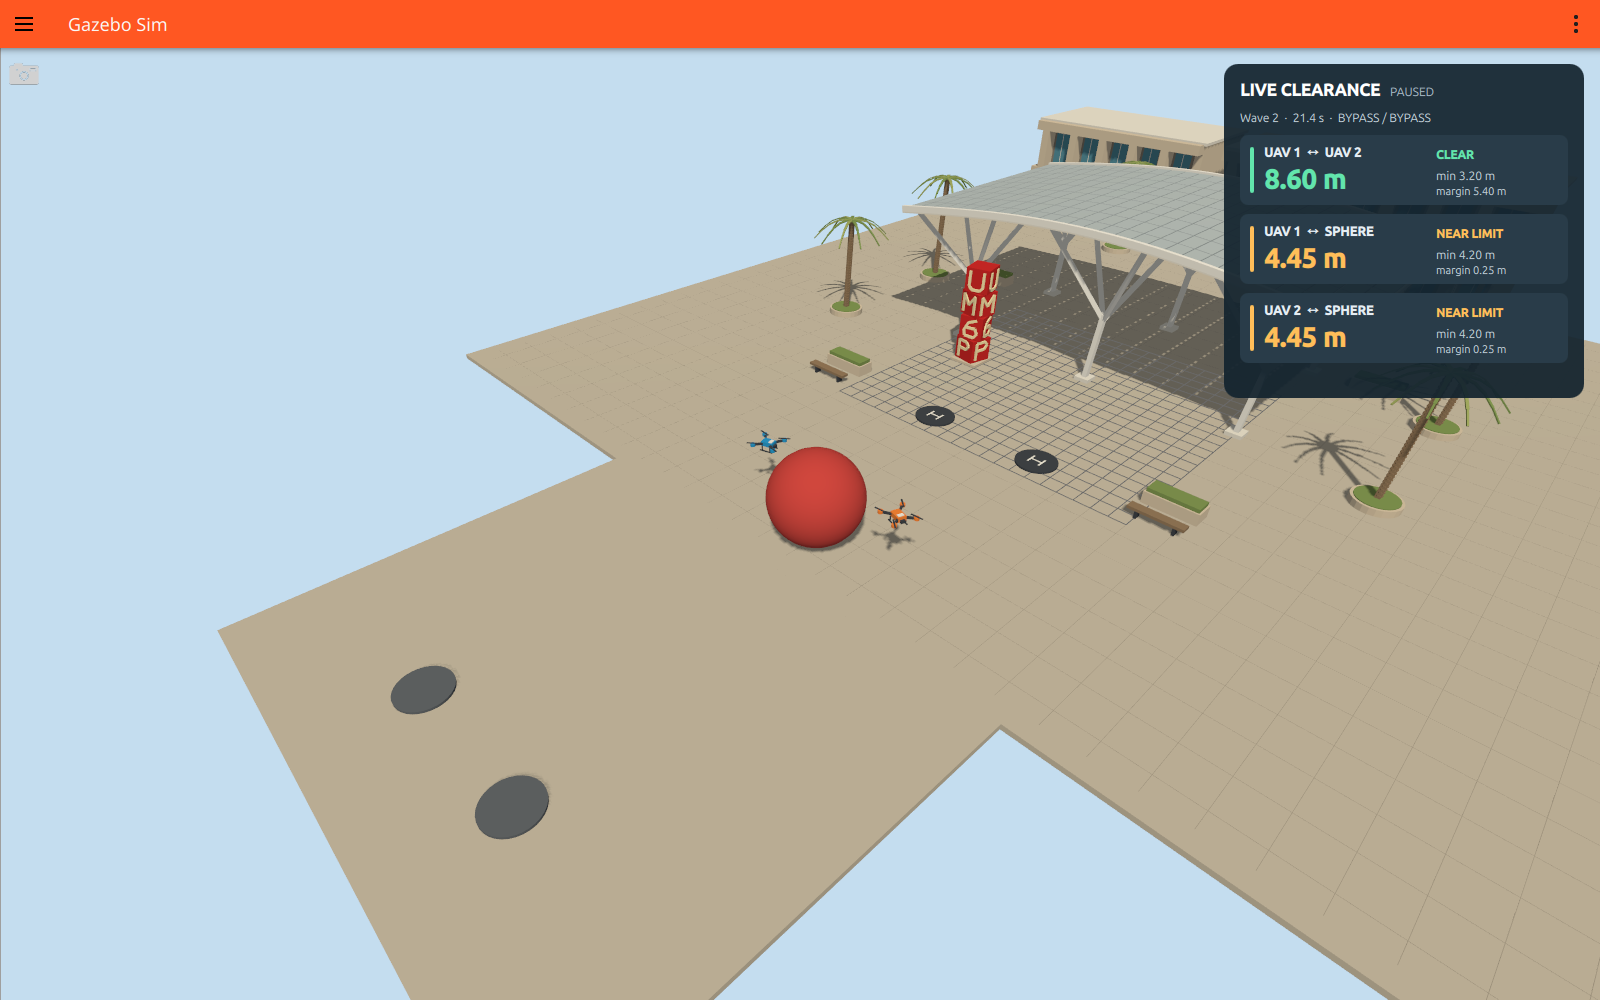
\includegraphics[width=.94\linewidth]{assets/obstacle.png}
\caption{Actual Gazebo Wave-2 rendering. Both vehicles pass close to the fixed sphere. The obstacle counters turn orange while the required clearance remains satisfied.}
\end{figure}

\section{Code lesson 4: connect the model to Gazebo}
\texttt{CampusKinematics.cc} is a small C++ system plugin. \texttt{Configure} reads the wave number, prepares a telemetry publisher and optionally opens a trace file. \texttt{PreUpdate} locates the two model entities, returns immediately while paused, validates the 0.02 s step, checks for unexpected external pose changes and applies an accepted joint movement. \texttt{PostUpdate} reads the entity poses back and publishes state.

The plugin writes both model poses in one simulator update thread. It does not send asynchronous independent movement commands to two nodes. The Gazebo dynamic-pose stream carries those changes to the renderer. No Physics system, motor model, sensor system or flight controller is loaded. Simulation time advances because the demonstration clock is running; it need not imply force integration.

The generated worlds reuse installed campus meshes. Only UAV static flags change in those separate worlds; destination pads, a paved extension and the optional sphere are added. The extension is 26 m wide and 20 m long, at ground height, covering $y=-45$ to $-25$; it joins the original courtyard. Existing buildings, pergola, landmark and landscaping are unchanged. The original world is untouched. \texttt{demo.launch.py} resolves installed package locations, loads the shared library and starts a one-way telemetry bridge. There is no ROS motion-command topic.

Working directory: delivery root. Prerequisite: stopped demonstration and an intentional edit to the world-generation recipe. Purpose: regenerate its two SDF files and reinstall changes. Expected result: two worlds generated, then a successful build. This is unnecessary for ordinary launching.
\begin{lstlisting}
python3 common/scripts/generate_demo_worlds.py
bash scripts/build.sh
\end{lstlisting}
When editing constants, reconcile the motion header, generated world geometry and independent verification thresholds. Their independent checks are intended to catch inconsistency. Do not loosen a test merely to hide an unsafe route.

\section{Code lesson 5: the live clearance display}
The upper-right panel belongs to Gazebo itself. \texttt{ClearancePanel.cc} receives the same state message that is bridged to ROS. Its transport callback queues a Qt GUI-thread update; \texttt{ClearancePanel.qml} formats the latest distances. The panel follows the right edge as the window changes size. It shows one counter in Wave 1 and three in Wave 2. The C++ capture service saves the actual full Gazebo window, including the panel.

Each large value is a center-to-center distance. The pair minimum is 3.20 m, which includes both 1.20 m vehicle bounds and 0.80 m required surface gap. Each sphere minimum is 4.20 m, including the 2.40 m obstacle radius, 1.20 m vehicle bound and 0.60 m required gap. The smaller margin is the displayed distance minus that minimum. These definitions belong here in the guide; the screen uses concise labels.

\begin{figure}[htbp]\centering
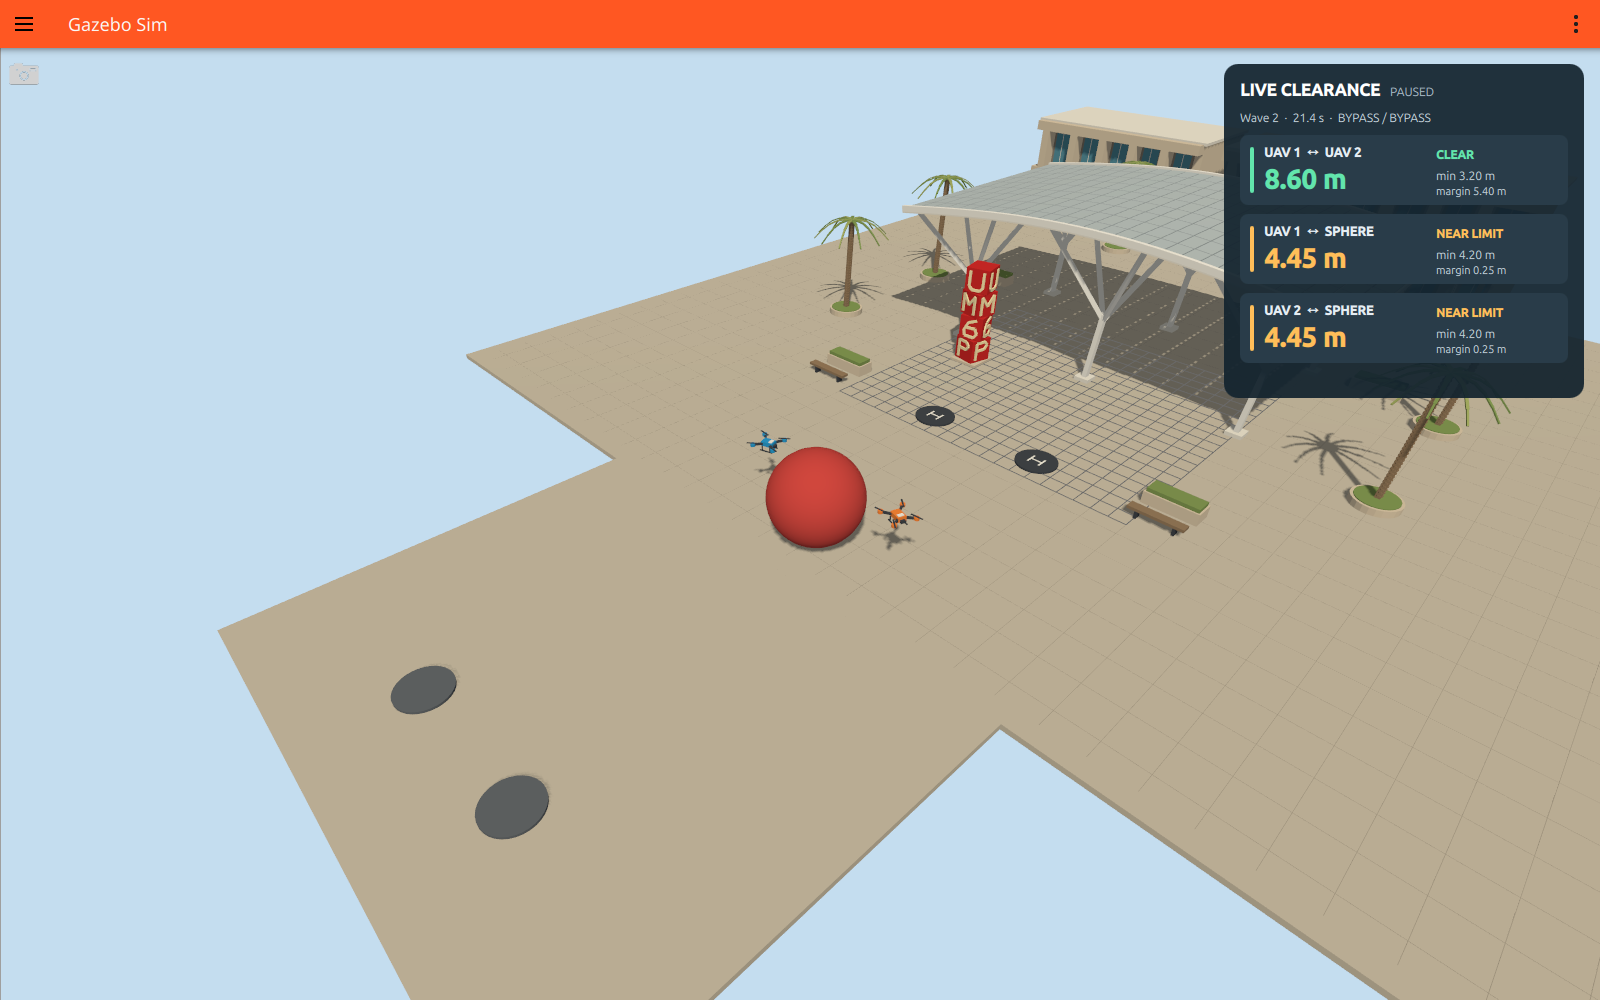
\includegraphics[width=.52\linewidth,trim={917.885bp 451.444bp 11.999bp 47.994bp},clip]{assets/obstacle.png}
\caption{Enlarged detail from the actual screenshot above. Both sphere distances are orange and remain above the 4.20 m minimum. This is a crop of Gazebo evidence, not a synthetic interface.}
\end{figure}

A margin of at least 0.80 m is green. A nonnegative margin below 0.80 m is orange. A negative margin is red. Color is accompanied by CLEAR, NEAR LIMIT or VIOLATION text, so color alone is not required to interpret it. Data older than 1.5 wall-clock seconds becomes gray and shows NO LIVE DATA. A paused scene still publishes stationary telemetry, allowing the panel to remain live without advancing time.

To understand the code, follow one message: the system reads the two executed model positions, adds the body-center offset when computing obstacle distances, serializes the values, and publishes them. The GUI parses the message, selects its wave-dependent row count, then evaluates each row's margin. It neither commands UAVs nor changes the acceptance guard. Red behavior is tested using synthetic QML input in an isolated test, without moving a Gazebo vehicle into danger.

Working directory: delivery root after a successful build. Purpose: exercise the motion core and the actual QML threshold functions without launching Gazebo. Expected result: two completed core cases and a JSON PASS with 20 panel cases. The offscreen Qt setting applies only to this widget test, not to a claim of software-rendered Gazebo verification.
\begin{lstlisting}
bash scripts/verify_unit.sh
\end{lstlisting}

\section{Verification and actual results}
Working directory: delivery root. Prerequisites: build succeeded and no other demonstration is running. Purpose: run a bounded test with its own isolated Gazebo partition and ROS topic/node namespace. Expected result: a JSON result with PASS, mission completion, measured minimum distances and clean exit. Each wrapper enforces a 150-second wall-time timeout. Output defaults to a new timestamped evidence directory.
\begin{lstlisting}
bash scripts/verify_demo.sh 1 headless
bash scripts/verify_demo.sh 2 gui
\end{lstlisting}
Run these sequentially. The GUI test saves a real screenshot at a paused midflight point. It verifies initial pause at zero time, starts motion, pauses during flight, checks unchanged positions/time, resumes, checks both landings, compares rendering poses to telemetry, checks ROS clock delivery and stops the launch owner. It then recomputes interval clearances from the full trace. The trace is actual execution evidence; the screenshot alone is not proof of safety.

\textbf{September 20 cross-talk correction.} A user Demo-2 failure log contained a wave=1 state received from a concurrently opened Demo 1. The old verifier shared ROS topics even though it isolated Gazebo. The corrected harness remaps state and clock to a unique ROS namespace and checks scenario identity. A paused-state barrier requires a new sample at or beyond the latest observed tick, then the original exact pose/time equality assertion remains in force. A regression test runs Demo 2 alongside a separate paused Demo 1. It saves all received states for diagnosis. Manual launch commands remain unchanged.

The automated verifier owns and closes its scene; it is not a presentation launcher. Failure cleanup is expected and is not itself a crash in the manual demo.

Early diagnostics are preserved separately from the final runs. One clean-copy diagnostic could not obtain the scene service response through the Python binding; bounded command-line service exchange resolved this. The first headless diagnostic completed Wave 1 but failed its final check because the scene-description service retained initial poses. The corrected harness uses \texttt{dynamic\_pose/info}, the renderer's motion stream. That diagnostic is retained as FAIL rather than silently relabeled. Final results and clean-copy checks are listed in \path{evidence/VERIFICATION_CURRENT.md}; they govern the tested scope.

Standalone core checks exercise crossing segments, a sphere-crossing segment, deterministic replay and timeout failure. The final GUI tests additionally establish actual rendering, exact entity count, pause/resume behavior, ROS message exchange and clean termination. A new-directory build checks installed-path portability; this does not establish fresh-OS provisioning.

\begin{center}\small\begin{tabular}{lrr}\toprule
Observed quantity & Wave 1 & Wave 2\\\midrule
Completion simulation time (s) & 51.92 & 54.22\\
Minimum UAV center distance (m) & 3.531609 & 3.530266\\
Minimum sphere-center distance (m) & not applicable & 4.366646\\
Yield duration (s) & 4.26 & 4.86\\
Pause/resume and renderer checks & PASS & PASS\\
Clean exit code & 0 & 0\\\bottomrule\end{tabular}\end{center}
These are observed GUI results, not illustrative outputs. All interval checks passed. The UAV-pair requirement is 3.2 m and the sphere-center requirement is 4.2 m. Wall-clock duration may differ with rendering load and inspection pauses.


\section{Visual Studio Code and troubleshooting}
Open the delivery root with File $>$ Open Folder. Use Terminal $>$ New Terminal for Terminal A and create a second terminal for control commands. Use the same commands as above. The included tasks provide build, parked campus, both demos and start/pause shortcuts. The two-terminal commands are the simplest recording workflow. Interactive VS Code UI itself is not a tested runtime route.

\textbf{No movement:} the scene starts paused. Issue start from another terminal in the same partition. Wait three simulation seconds after start. Check that the demo world, not the original paused world, is open.

\textbf{Control service timeout:} confirm the launch is still running and both terminals use the same Gazebo partition. Close a conflicting scene. Do not target the old world or change system security settings.

\textbf{Library or package missing:} rebuild, then launch through the wrapper so both ROS and the local install are sourced. A source directory alone does not make an installed package discoverable. Do not copy an old install directory to a new path.

\textbf{Blocked route/FAILED:} retain the trace and failure result. Inspect waypoint, radius, corridor and sphere consistency. An arbitrary new layout is not guaranteed to work with this two-scenario heuristic.

\textbf{Unexpected pose modification:} another tool changed a UAV entity. Close the scene and restart it. Do not use transform tools or additional controllers alongside this demo.

\textbf{Blank GUI:} use the same desktop graphics session as the working original campus. This task used hardware rendering; software/EGL behavior remains unverified. No graphics-driver replacement is part of recovery.

Safe cleanup: stop Terminal A first. The build, install, log and .runtime directories inside this workspace are disposable. Preserve source, evidence, tutorials and checkpoints. Avoid broad process-kill commands that could affect unrelated work.

\section{Rebuild this guide and recover work}
Working directory: delivery root. Prerequisites: latexmk or Tectonic on PATH, plus Poppler for inspection; the original guide documents optional TeX dependencies. Purpose: regenerate imported source listings and compile this exact guide. Expected result: \path{tutorial/02_Two_UAV_Kinematic_Demos_Coding_and_Verification.pdf} and PDF metadata.
\begin{lstlisting}
bash scripts/build_kinematic_tutorial.sh
\end{lstlisting}
The appendix imports maintained source directly. The generated vertex tables remain in the original campus package and need not be copied into this second guide. TeX dependencies may download at documentation-build time; scene runtime has no such requirement. PDF binary equality across TeX versions is not promised.

On resume, read the current checkpoint, check which source and evidence files exist and compare hashes before rebuilding anything. Preserve intervening user edits. Do not repeat completed experiments just to fill a log. Save progress after meaningful milestones and before expensive operations; a cache or session may not survive a later invocation.

The original paused environment was published first as GitHub \href{https://github.com/ismo-idi/CCBO_Model1/commit/3e8f51848bd6057005a782b31da2a25c9c7ca268}{commit 3e8f518}. The current scientific context is Model 0-D v1.6, with its own three-attempt campaign and exact-oracle limitations. Those outcomes belong to their original evidence. This new showcase neither executes nor certifies TCC/Sun--Sun, and does not replace its benchmark.

\section*{Official references}
\addcontentsline{toc}{section}{Official references}
\begin{enumerate}
\item \href{https://gazebosim.org/api/sim/8/createsystemplugins.html}{Gazebo Sim 8: creating system plugins}, update interfaces, pause/time semantics and plugin loading.
\item \href{https://gazebosim.org/api/sim/8/classgz_1_1sim_1_1EntityComponentManager.html}{Gazebo EntityComponentManager}, entity/component access.
\item \href{https://docs.ros.org/en/jazzy/p/ros_gz_bridge/}{Official ros\_gz\_bridge documentation}, message bridge configuration.
\item \href{https://gazebosim.org/api/gui/8/plugins.html}{Gazebo GUI 8 plugins}, native C++/QML widgets and plugin search paths.
\item Project Model 0-D v1.6 and Decisions 03/04 at the repository commit recorded in the delivery references. These provide the scoped geometric formulation; this guide adds engineering scenario choices.
\end{enumerate}

\section{Where to edit each part}
\path{demo/demo_1_no_obstacle/} contains Demo 1's package, route input, expected milestones and media. \path{demo/demo_2_static_sphere/} contains the corresponding Demo 2 files. \path{common/src/um6p_demo_core/} contains Motion.hh, Routes.hh, the Gazebo system, native clearance panel and common bridge/launch configuration. \path{common/tests/} holds shared integration and geometry checks. Campus meshes exist only in the description package under \path{campus_environment/}.

To study or extend a route, read its two lines of x y z triplets, follow the generator into the SDF plugin fields, then follow Routes.hh into Motion. Rebuild after generation. Do not add a second copy of shared motion logic to a scenario package. Any change in routes, bounds, vehicle count or geometry requires new clearance tests; the current expected milestone files deliberately detect motion changes.
